
\chapter{Supplementary Material for Repairing the Surface of InAs-based Topological Heterostructures}
\section{Fabrication Details}
All devices presented here were from a single wafer, grown via molecular beam epitaxy with a \SI{10}{\nano\meter} aluminum cap grown \emph{in-situ}. Hall bars are defined in PMMA using electron-beam lithography. Mesas were etched using a chemical wet etch process, which includes an Al etch using Transene-D, heated to \SI{47.8}{\celsius}, and etched for \SI{11}{\second}, followed by three \SI{11}{\second} rinses in DI water. The InAs is then etched in dilute phosphoric acid (50:5:1 \ce{H2O}:\ce{H3PO4}:\ce{H2O2}) for \SI{95}{\second}, to a depth of $\sim \SI{180}{\nano\meter}$, again followed by three \SI{11}{\second} rinses in DI water. Finally, a \SI{6}{\second} Transene-D dip is used to remove any overhanging Al, followed by three \SI{11}{\second} rinses in DI water. The resist was stripped quickly after completion of the final etch using Acetone.

Aluminum is removed from the surface of the mesa, except at contacts, using Transene-D heated to \SI{47.8}{\celsius} and etched for \SI{11}{\second}, followed by three \SI{11}{\second} rinses in DI water. The resist was stripped quickly after completion of the final etch using Acetone.

Surface treatment and oxide growth is performed in the Picosun R200 ALD tool, fitted with a load-lock, a remote plasma source and an ozone generator. The stage temperature is set to \SI{200}{\celsius} and a constant flow of \ce{N2} gas is used to purge the tool, including during the treatment steps.

For the ArH plasma treatment, the ArH plasma is generated with an Advanced Energy Litmas™ RPS 3001 remote plasma source at \SI{1000}{\watt} source power, and a \SI{20}{\second} pulse is applied 6 times, with a \SI{30}{\second} gap between each run. We note that during this process \ce{N2} gas continues to flow through the process chamber.

For the TMA reduction treatment, TMA is pulsed for \SI{1.0}{\second}, with a \SI{30}{\second} purge between cycles. This is repeated 10 times prior to oxide growth.

Oxide growth is performed \emph{in-situ} using 170 cycles of TMA and either \ce{H2O} or \ce{O3}, following a standard recipe for oxide growth.

\section{Measurement}
\label{sec:surf_mulberry}
Measurements are taken in a BlueFors LD400 dilution refridgerator, fitted with a wide-bore \SI{2}{\tesla} solenoid, with a base temperature of \SI{7}{\milli\kelvin}. A custom Cryo-CMOS based multiplexer is used to map each of 32 input DC lines to 5 outputs, for a total of 160 DC lines, and is used to allow measurement of up to 10 Hall bars in a single cool-down. The CMOS is fabricated commercially on the AMS \SI{0.35}{\micro\meter} process. A schematic of this setup is shown in Fig.~\ref{fig:surf_cmos}.

\begin{figure}[h]
    \includegraphics[width=0.8\linewidth]{FigureS1}
    \caption[Measurement multiplexing setup]{(a) Schematic of a single cell of the multiplexing chip. Each input is multiplexed to 5 outputs, allowing for a total of 160 DC lines to be measured using 32 lines. (b) Image of the multiplexing chip. (c) Mounted measurement board, with four samples mounted around the bottom of the board.}
    \label{fig:surf_cmos}
\end{figure}

Measurements are taken with a lockin, with a \SI{10}{\nano\ampere} constant current applied across the device through a \SI{100}{\mega\ohm} resistor. The top gate voltage is applied using a Yokogawa GS200 voltage source.

\clearpage
\section{Density and Mobility for all Treatments}
\label{sec:all_treat}
\vfill
\begin{figure}[h]
    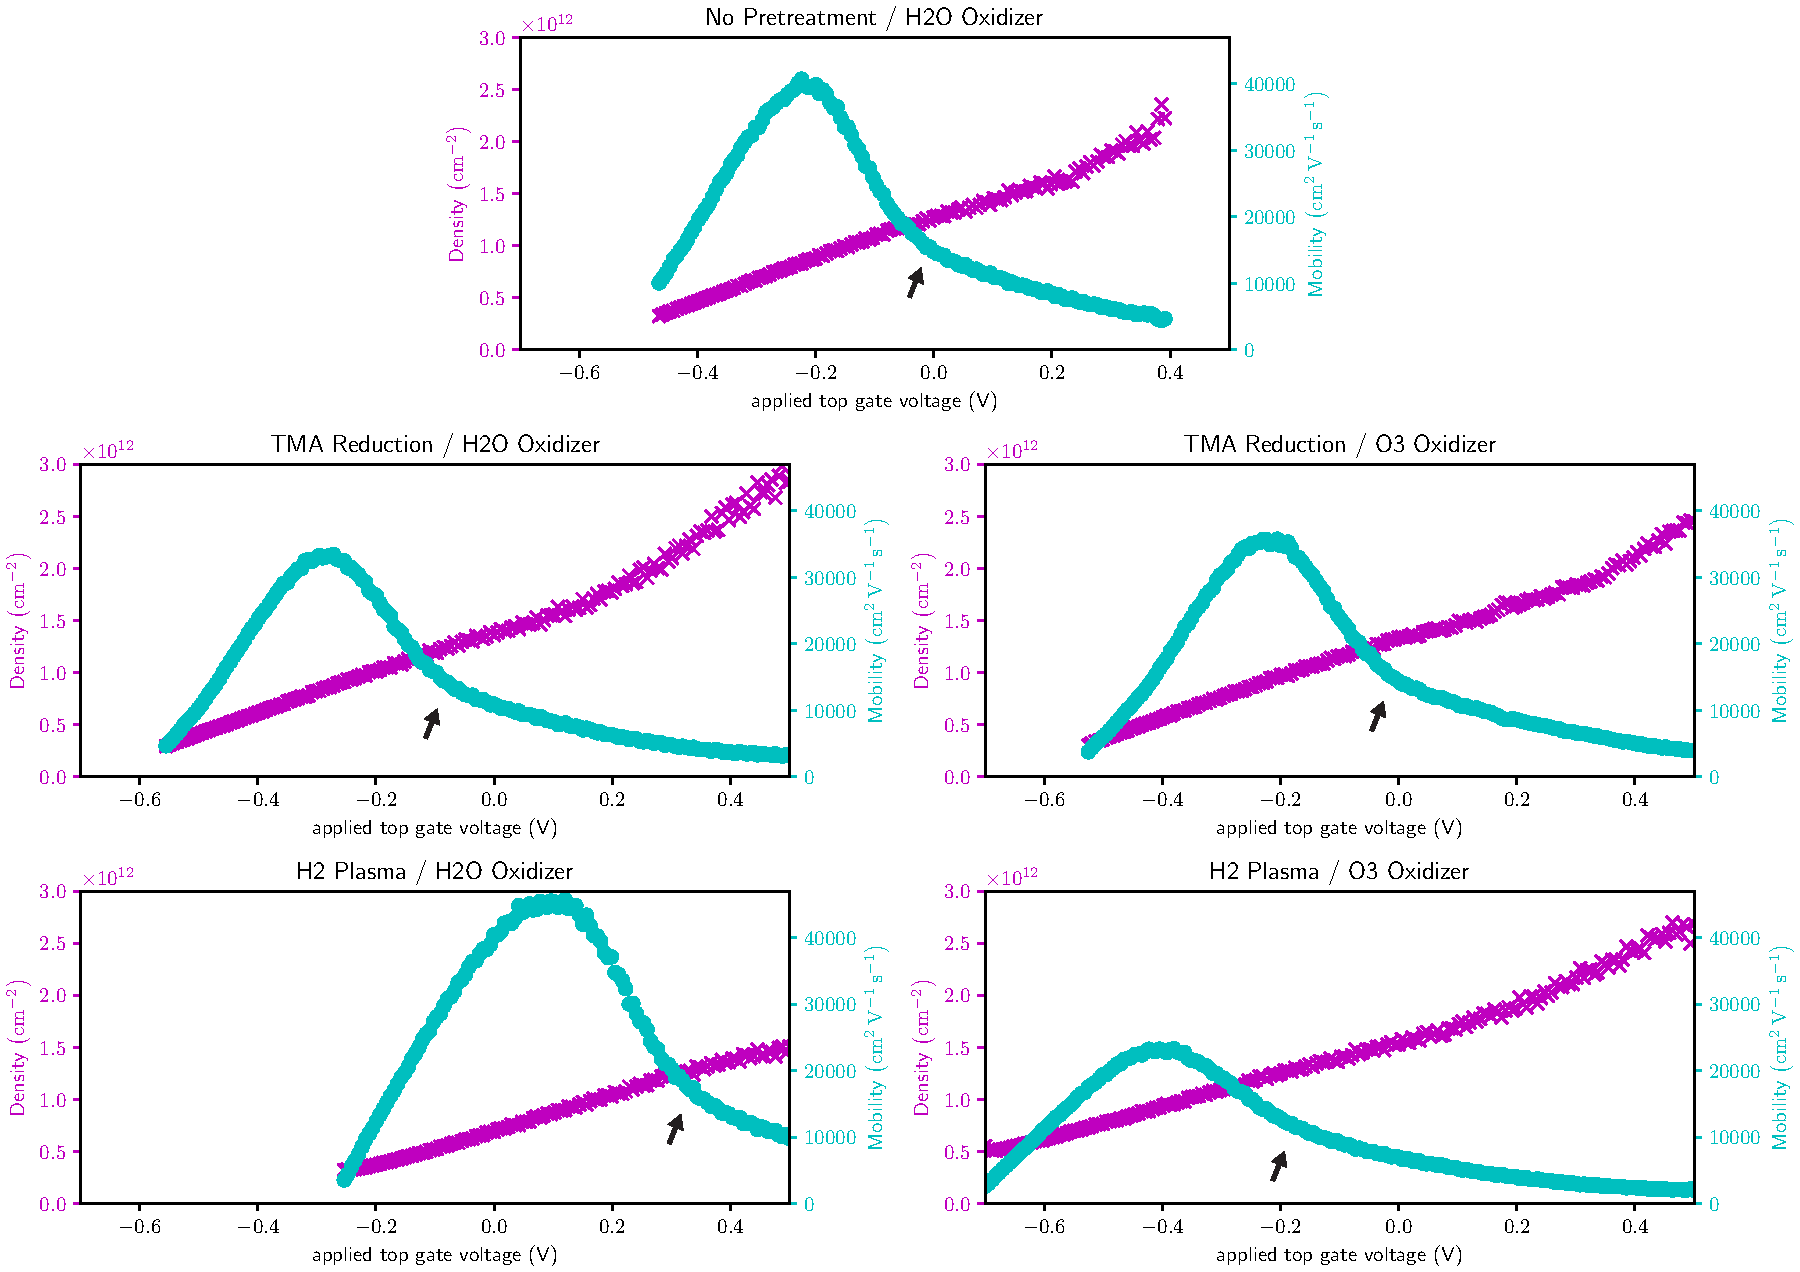
\includegraphics[width=\linewidth]{FigureS3}
    \caption[Density/Mobility for all Treatments]{The density and mobility traces as gate voltage is swept for all surface treatments. The location of second subband population is marked with an arrow on each trace.}
    \label{fig:surf_allt}
\end{figure}
\vfill

\clearpage
\section{Density at Peak Mobility}
\label{sec:surf_mobden}
\vfill
\begin{figure}[h]
    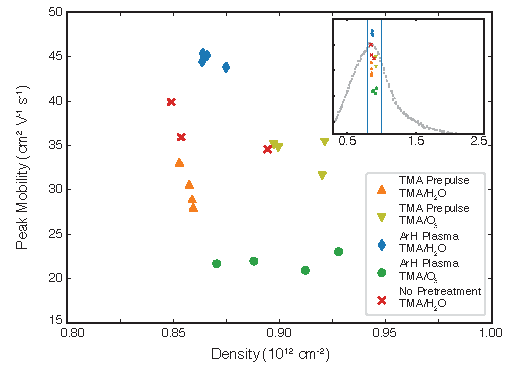
\includegraphics[width=0.65\linewidth]{FigureS2}
    \caption[Location in density of peak mobility]{The location in density that peak mobility occurs, for samples taken near the center of the growth wafer. Samples grown with ozone are shifted to the right relative to samples grown with water.}
    \label{fig:surf_mobden}
\end{figure}
\vfill